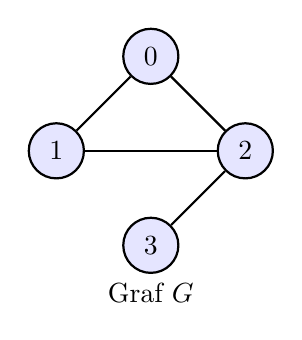
\begin{tikzpicture}[
  vnode/.style={circle, draw, minimum size=7mm, inner sep=0pt, fill=blue!10},
  thick
]
  % Graf pro ukázku reprezentace
  \node[vnode] (0) at (0, 1.2) {0};
  \node[vnode] (1) at (-1.2, 0) {1};
  \node[vnode] (2) at (1.2, 0) {2};
  \node[vnode] (3) at (0, -1.2) {3};
  \draw (0) -- (1);
  \draw (0) -- (2);
  \draw (1) -- (2);
  \draw (2) -- (3);
  \node at (0, -1.8) {Graf $G$};
\end{tikzpicture}
\par\medskip
Vyjádření tohoto grafu $G$ pomocí obou struktur:
\par\medskip
\begin{minipage}[t]{0.45\textwidth}
\centering
\textbf{Matice sousednosti $A_G$}
$$\begin{pmatrix}
0 & 1 & 1 & 0 \\
1 & 0 & 1 & 0 \\
1 & 1 & 0 & 1 \\
0 & 0 & 1 & 0
\end{pmatrix}$$
\end{minipage}
\begin{minipage}[t]{0.45\textwidth}
\centering
\textbf{Seznam sousedů}
\begin{itemize}[leftmargin=2em, itemsep=0pt]
    \item[\textbf{0:}] $\to 1 \to 2$
    \item[\textbf{1:}] $\to 0 \to 2$
    \item[\textbf{2:}] $\to 0 \to 1 \to 3$
    \item[\textbf{3:}] $\to 2$
\end{itemize}
\end{minipage}
\par\medskip
\textit{Obrázek 3.1: Graf $G$ a jeho ekvivalentní vyjádření v paměti modelu RAM.}